Обучение игре в шахматы является одним из популярных подходов к формированию стратегического мышления.

В работе \cite{Adam2024} проведен анализ в соревнованиях проприетарного решение ChatGPT демонстрировал рейтинг Эло 1600,
соответствующий начальном уровню игрока в шахматы \cite{elo1967proposed}. Открытое решение \cite{feng2024chessgpt} использует архитектуру декодера для 


\begin{figure}[h]
    \centering
    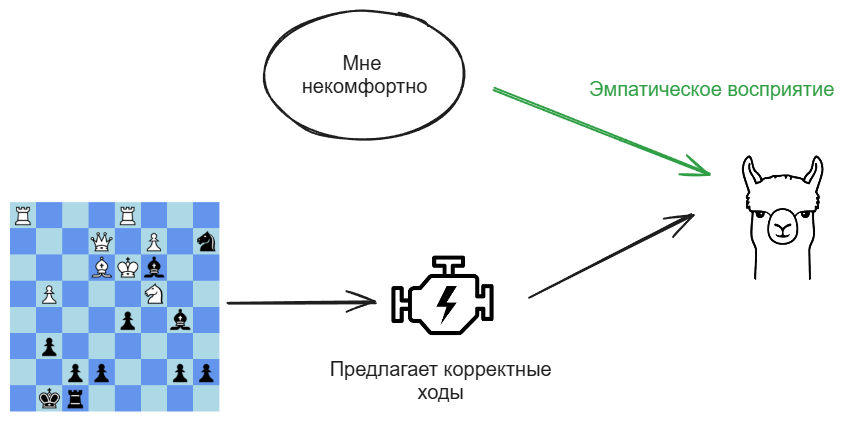
\includegraphics[width=0.5\textwidth]{assets/work/games/llama-chess.excalidraw.png}
    \caption{Планирование игры выполняется шахматным движком Stockfish. Языковой ассистент комментирует игру и следит за сложностью}
    \label{chess}
\end{figure}

Исходя из этого был подготовлен совместный подход, 
использующий открытый шахматный движок StockFish \cite{acher2016large} для ранжирования наилучшего хода. 

Таким образом, интеллектуальный ассистент отвечает за эмпатическое понимание пользователя и коррекцию сложности,
а шахматный движок предлагает ход согласно уровню игры.



Растровый рисунок использует сеточное заполнение цветом. Из-за этого при изменение разрешения изображения картинка приобретает
резкий вид, связанный с наблюдением резкой сетки заместо плавного изображения.

Тем не менее такой вид искусства популярен в силу простоты освоения и восприятия. Интерактивная игра предлагает 

Для отображения используется открытая диффузионная модель \ref{diffusion} для составления рисунка по текстовому запросу. 

Для выполнения рисунка она получает запрос на английском языке, лаконично описывающий стиль рисования и объекты на изображении.
В силу случайности генерации пользователь может подобрать для себя наиболее интересный вариант изображения.

Модель дополнительно снабжена фильтром цензуры, позволяющей избегать неэтичного рисунка \cite{radford2021learning}.

\begin{figure}[h]
    \centering
    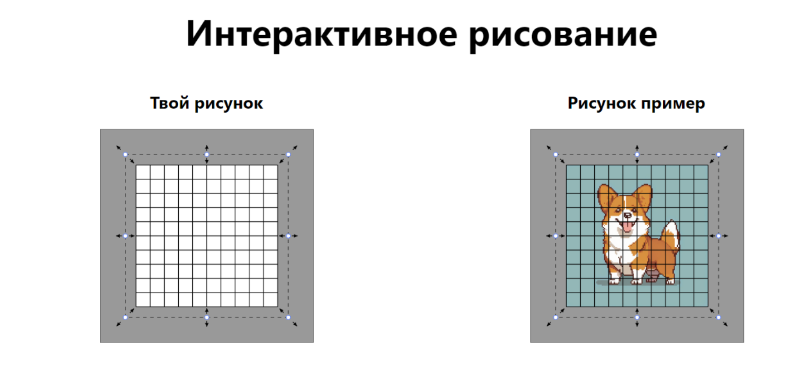
\includegraphics[width=0.5\textwidth]{assets/work/games/interface.excalidraw.png}
    \caption{Сложность задания задается организацией рисунка}
    \label{draw}
\end{figure}


Ассистент выполняет задачи \begin{itemize}
    \item транслирует запрос пользователя на русском языке на английский для генерации
\end{itemize}



Уровень сложности регулируется путем изменения композиции и наличия фона.




\begin{figure}[h]
    \centering
    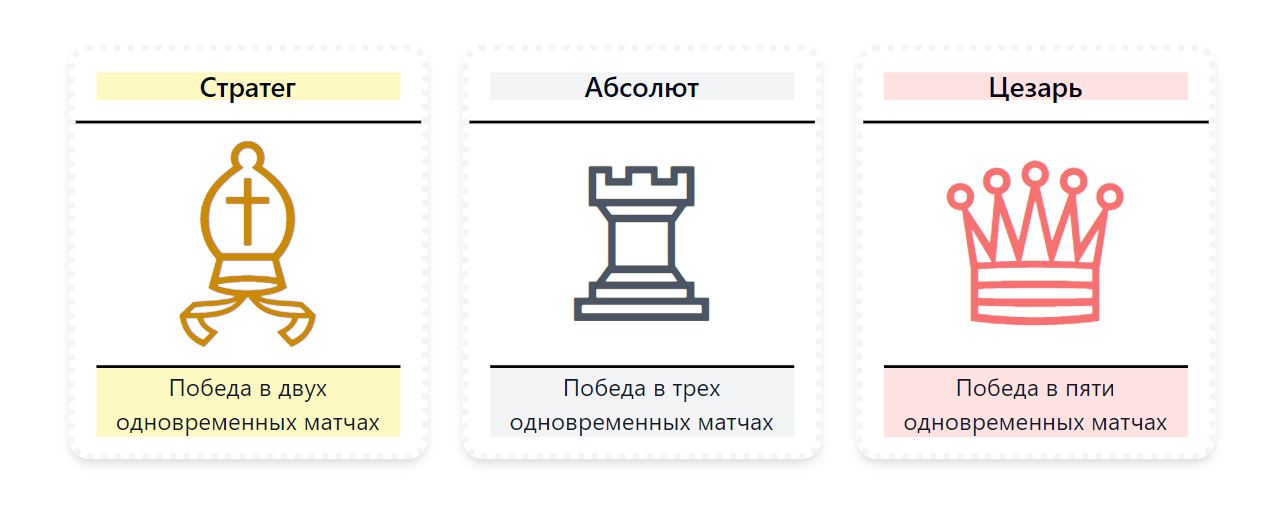
\includegraphics[width=0.5\textwidth]{assets/work/games/achieve.png}
    \caption{}
    \label{chess}
\end{figure}








